\documentclass[tikz,border=3pt]{standalone}
\usepackage[utf8]{inputenc}
\usepackage[T1]{fontenc}
\usepackage{lmodern}
\renewcommand{\familydefault}{\sfdefault}
\usepackage{sansmath}\sansmath
\usepackage{chemfig}
\usepackage{pgfplots}\pgfplotsset{compat=1.18,/pgf/number format/use comma,/pgf/number format/1000 sep={.}}
\usetikzlibrary{arrows.meta,calc,positioning,decorations.pathmorphing,patterns}
% paleta del sitio
\definecolor{nar}{HTML}{E8680C}\definecolor{narc}{HTML}{FFB35C}\definecolor{hielo}{HTML}{FFF3E8}
\definecolor{tinta}{HTML}{1D1D1F}\definecolor{gris}{HTML}{6E6E73}\definecolor{lila}{HTML}{7C5CF0}
\definecolor{azul}{HTML}{2F6FD6}\definecolor{menta}{HTML}{17A673}\definecolor{coral}{HTML}{E8342A}
\begin{document}
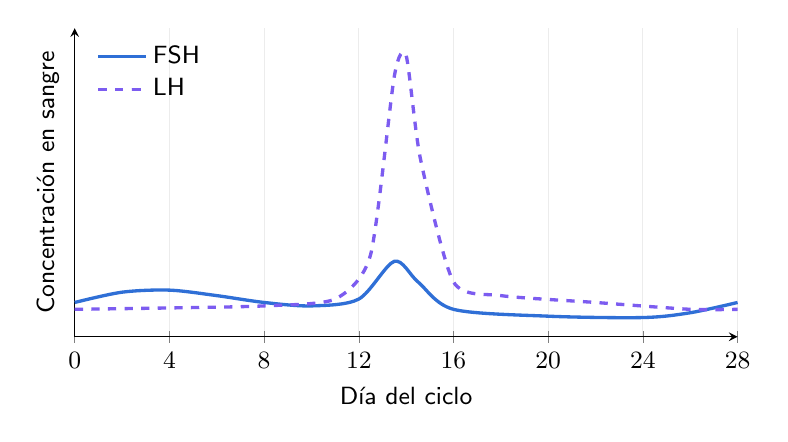
\begin{tikzpicture}[font=\small]
\begin{axis}[width=10cm,height=5.5cm,xmin=0,xmax=28,ymin=0,ymax=45,axis lines=left,ytick=\empty,xtick={0,4,...,28},
 xlabel={Día del ciclo},ylabel={Concentración en sangre},grid=major,grid style={gray!15},clip=false,
 legend cell align=left,legend style={draw=none,fill=none,at={(0.02,0.98)},anchor=north west}]
\addplot[azul,very thick,smooth] coordinates {(0,5)(2,6.5)(4,6.8)(6,6)(8,5)(10,4.5)(12,5.5)(13.5,11)(14.5,8)(16,4)(20,3)(24,2.8)(26,3.5)(28,5)};
\addlegendentry{FSH}
\addplot[lila,very thick,smooth,tension=0.4,dashed] coordinates {(0,4)(4,4.2)(8,4.5)(11,5.5)(12.5,12)(13.5,38)(14,41)(14.6,26)(16,8)(18,6)(22,5)(26,4)(28,4)};
\addlegendentry{LH}
\end{axis}
\end{tikzpicture}
\end{document}
